\section{Teoria dei Grafi}
La teoria dei grafi è una branca della matematica, nata nel 1700 con Eulero, che consente di descrivere le relazioni che intercorrono tra un insieme di oggetti.\\
Il grafo è lo strumento attraverso il quale tali relazioni possono essere espresse ed organizzate. Infatti, il grafo, consiste di oggetti chiamati \textit{nodi} e relazioni tra coppie di questi oggetti detti \textit{archi}; nodi connessi tra loro da un arco sono detti \textit{vicini} o \textit{adiacenti}.\\

\begin{figure}[h!]
	\centering
	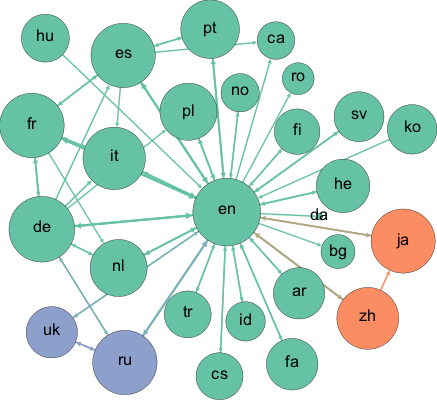
\includegraphics[scale=.5]{img/Wikipedia_multilingual_network_graph_July_2013.png}
	\caption{Wikipedia Multilingual Network Graph (July 2013)}
\end{figure}
\newpage
La relazione tra una coppia di nodi può essere di due tipi:
\begin{itemize}
	\item Simmetrica: l'arco connette i nodi con un collegamento bidirezionale ed è detto \textit{indiretto}. Un grafo costituito di soli archi indiretti è anch'esso detto indiretto.
	\item Asimmetrica: l'arco connette i nodi con un collegamento unidirezionale ed è detto \textit{diretto}. Un grafo costituito di soli archi diretti è anch'esso detto diretto.
\end{itemize}
\begin{figure}[h!]
	\vspace*{1cm}
	\begin{minipage}{0.45\textwidth}
	\centering
	\begin{tikzpicture}[-,>=stealth',shorten >=1pt,auto,node distance=2cm,
		thick,main node/.style={circle,draw,font=\sffamily\Large\bfseries}]
		\node[main node] (1) {1};
		\node[main node] (2) [below left of=1] {2};
		\node[main node] (3) [below right of=2] {3};
		\node[main node] (4) [below right of=1] {4};
		\path[every node/.style={font=\sffamily\small}]
		(1) edge node [left] {} (4)
		
		(2) edge node [right] {} (1)
		
		(3) edge node [right] {} (2)
		
		(4) edge node [left] {} (3);
		
	\end{tikzpicture}
	\caption{Grafo indiretto}
	\end{minipage}\hfill
% <-- needed to keep the imgs side by side
	\begin{minipage}{0.45\textwidth}
	\centering
	\begin{tikzpicture}[->,>=stealth',shorten >=1pt,auto,node distance=2cm,
		thick,main node/.style={circle,draw,font=\sffamily\Large\bfseries}]
		\node[main node] (1) {1};
		\node[main node] (2) [below left of=1] {2};
		\node[main node] (3) [below right of=2] {3};
		\node[main node] (4) [below right of=1] {4};
		\path[every node/.style={font=\sffamily\small}]
		(1) edge node [left] {} (4)
		
		(2) edge node [right] {} (1)
		
		(3) edge node [right] {} (2)
		
		(4) edge node [left] {} (3);
	\end{tikzpicture}
	\caption{Grafo diretto}
	\end{minipage}
\end{figure}
Un grafo può essere formalmente descritto come una coppia di insiemi \textbf{G = (V, E)}, dove V è l'insieme dei nodi ed E è l'insieme degli archi. Un arco e $\in$ E è rappresentato come un sottoinsieme di due elementi di V, $e = \lbrace u, v\rbrace$ per $u, v \in V$.\\
Le rappresentazioni atte a descrivere un grafo sono molteplici:
\begin{itemize}
	\item \textit{Rappresentazione grafica}: ad ogni nodo corrisponde una figura circolare sul piano e ad ogni arco (i, j) corrisponde una linea che che collega il nodo i al nodo j.
	\item \textit{Matrice di adiacenza}: matrice di dimensione $n \times n$, dove $n$ è il numero di nodi, il cui elemento (i, j) assume valore 1 se esiste l'arco tra il nodo i ed il nodo j, 0 altrimenti.
	\item \textit{Lista di adiacenza}: ad ogni vertice $v$ è associata la lista dei nodi ad esso vicini.
\end{itemize}
Negli anni, gli studi sulla teoria dei grafi hanno prodotto una quantità enorme di definizioni e teoremi, per cui, di seguito vengono descritti solamente i concetti necessari alla comprensione di questo lavoro di tesi.
\paragraph{Sottografo.} Un grafo H si dice sottografo di un grafo G se i vertici di H sono un sottoinsieme dei vertici di G e gli archi di H sono un sottoinsieme degli archi di G. Siano $G=(V, E)$ ed $H=(V_1, E_1)$ due grafi. H è un sottografo di G se e solo se $V_1 \subseteq V$ ed $E_1 \subseteq E$.
Un concetto particolarmente utile alla comprensione di questo lavoro è lo \textit{spanning subgraph}: uno spanning subgraph H di un grafo G è un sottografo che contiene tutti i vertici di G, cioé $V_1 = V$.
\paragraph{Grado di un nodo.} Il grado di un nodo $v$ è il numero di nodi ad esso adiacenti ed è indicato con \textit{deg(v)}.\\
In un grafo diretto, si distinguono due tipi di grado:
\begin{itemize}
	\item \textit{in-deg(v)}, il grado in ingresso del nodo \textit{v}, dato dal numero di archi in cui \textit{v} compare come nodo destinazione;
	\item \textit{out-deg(v)}, il grado in uscita del nodo \textit{v}, dato dal numero di archi in cui \textit{v} compare come nodo sorgente.
\end{itemize}
\paragraph{Cammino.} Un cammino è una sequenza di nodi, in cui ogni coppia consecutiva della sequenza sia connessa da un arco. Formalmente, un cammino è una sequenza di vertici $v_0, v_1, \cdots, v_n \in V$ tale che $\lbrace v_{i-1}, v_i\rbrace \in E, \forall 1\leq i \leq n$. Un cammino con almeno tre vertici distinti, i cui vertici di inizio e fine coincidono, è detto \textit{ciclo}.
\paragraph{Grafo connesso.} Un grafo è connesso se, per ogni coppia distinta di vertici (i, j), esiste un cammino da i a j.

\subsection{Grafo come modello della realtà}
I grafi hanno una grande utilità, in quanto consentono di astrarre le relazioni che intercorrono tra più oggetti, e di rappresentare tali relazioni in strutture su cui è possibile applicare modelli matematici. In \cite{easley2010networks} viene proposto un esempio reale: la Figura \ref{arpanet} rappresenta la struttura della rete Internet nel Dicembre del 1970, noto come ARPANET allora, composto solo da 13 macchine. I nodi rappresentano gli host, e vi è un arco tra due host se esiste una comunicazione diretta tra di essi.
\begin{figure}[h!]
	\centering
	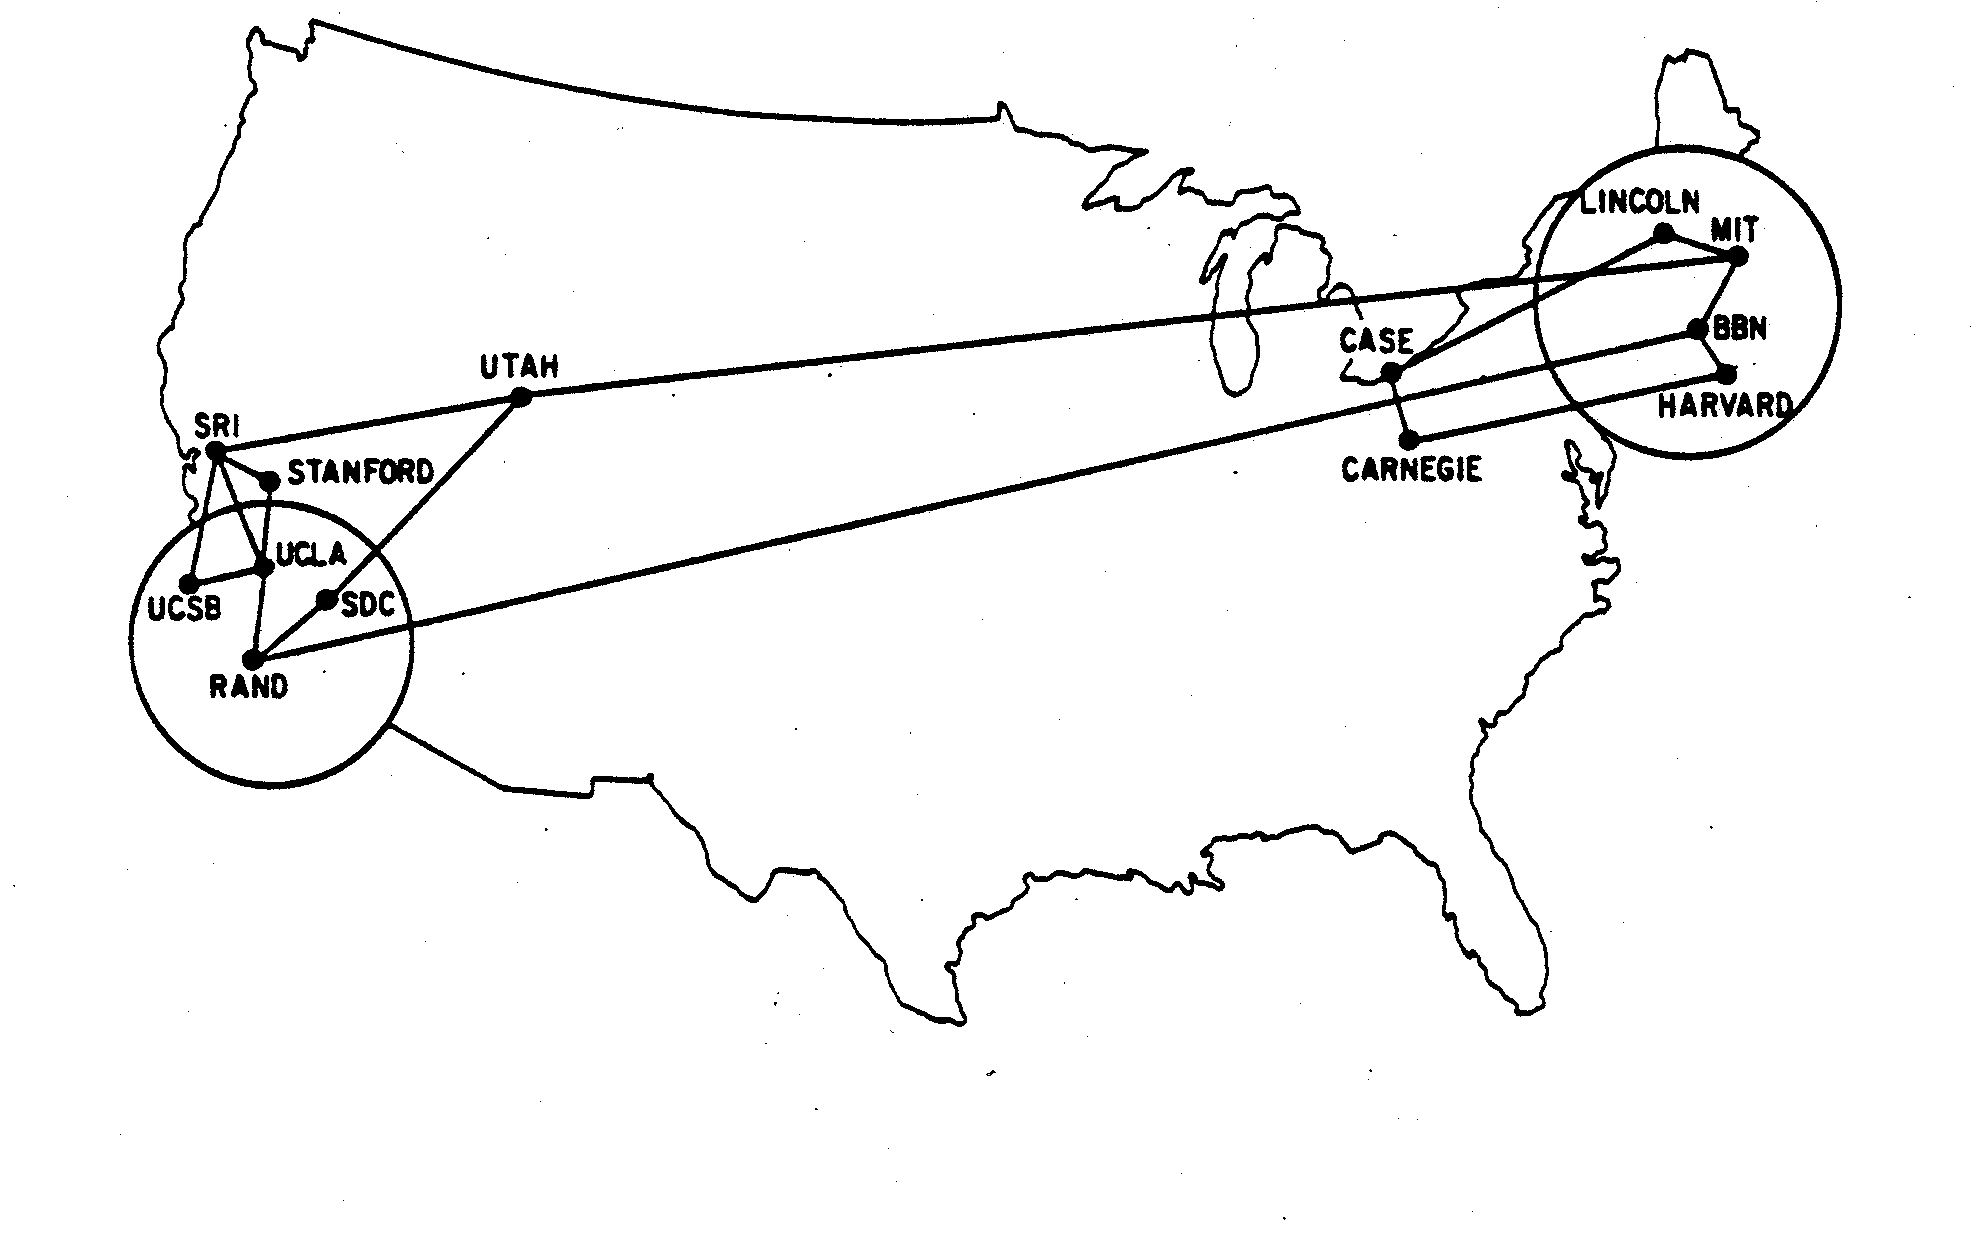
\includegraphics[scale=.7]{img/arpanetdec1970.jpg}
	\caption{ARPANET nel Dicembre 1970}
	\label{arpanet}
\end{figure}
Come è possibile intuire, la posizione geografica dei nodi non ha molta importanza, ma quel che conta è il come ogni nodo sia connesso agli altri. Infatti la figura \ref{arpanet_graph} mostra lo stesso grafo di ARPANET, attraverso una rappresentazione logica.
\begin{figure}
	\centering
	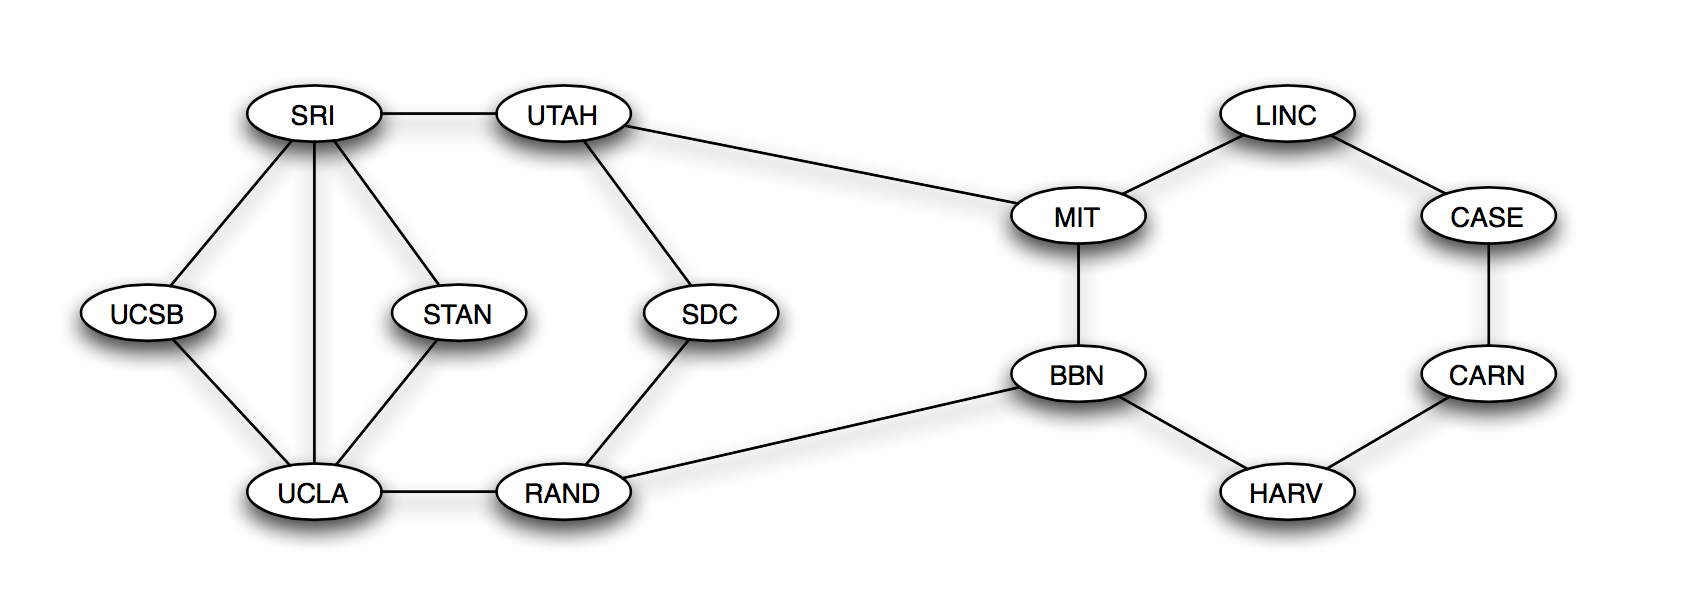
\includegraphics[scale=.5]{img/arpanetdec1970_graph.png}
	\caption{Grafo di ARPANET nel Dicembre 1970}
	\label{arpanet_graph}
\end{figure}
Il grafo di ARPANET mostrato in precedenza è un esempio di \textit{\textbf{communication network}}, i cui nodi sono computer o altri dispositivi capaci di inviare messaggi mentre gli archi rappresentano i collegamenti diretti lungo i quali tali messaggi possono viaggiare. Ma questo è solamente uno dei tipi di rete che possiamo avere.\\
Le \textit{\textbf{social network}} i cui nodi sono persone o gruppi di persone, ed i cui archi rappresentano un tipo di interazione (amicizia, inimicizia, ecc.), sono reti massive che al giorno d'oggi comprendono gran parte della popolazione mondiale.
\subsection{Complex Networks}
%wiki seems good


\section{Modello di Ising}
\subsection{Partition Function}

\section{Cenni di probabilità e statistica}

\section{Processi Markoviani}
\subsection{Irriducibilità e periodicità}
\subsection{Distribuzione stazionaria}
\subsection{Catena di Markov Monte Carlo}

\section{Algoritmi di approssimazione}